% !TEX root = pfe-book3.tex
%!TEX TS-program = pdflatex
%!TEX encoding = UTF-8 Unicode


\cleardoublepage
%\mainmatter
\chapter{Electromagnetic Fields}
\label{ch-05}

\section{Maxwell's Equations}
By the fifties of last century, much information had accumulated on electricity and magnetism. It was disconnected in the main, however, sometimes contradictory and, in any case, did not fit into a single orderly system.


But a great deal was known. In the first place, physicists knew that electric charges at rest set up an electric field; secondly, that electric currents set up magnetic fields; and, thirdly, the results of Faraday's experiments were published and generally recognized. In them he proved that a variable magnetic field generates an electric current.

In those times, a number of scientists, and primarily Faraday, doubtlessly became convinced that some kind of events occur in the space surrounding electric currents and charges. This group of investigators supposed that magnetic and electric forces are transmitted from point to point. Attempts were widely made to draw diagrams, similar to a system of meshing gears, which could visually demonstrate the mechanism of the transmission of electric energy. But certain men of science advocated the theory of long-range interaction. They denied the physical process of transmitting electric and magnetic forces. They said that the concepts of a field and lines of force are to be treated as only geometric images that do not represent any possible kind of reality.

As has frequently occurred in the history of science, the truth turned out to be somewhere in the middle. Attempts to reduce electromagnetic phenomena to the motion of a special kind of matter -- the ether -- were found to be unsound. But, on the other hand, investigators that proposed that electromagnetic interaction is transmitted instantaneously from one charge or current to another were also wrong.

The famed Scottish physicist James Clerk Maxwell (1831-1879) published a work called \emph{On Faraday's Lines of Force} when he was only 26. As a matter of fact, this work already contained the laws he discovered. Several more years were required, however, for him to discard his mechanistic conceptions and to formulate the laws of an electromagnetic field in a form that requires no na\"ive graphical illustration.

In this connection Maxwell once said that for the benefit of people with different kinds of minds scientific truth should be presented in various forms and be regarded as equally scientific whether it is presented in the clear form and lively colours of physical illustration or in the simplicity and pallor of symbolic expression.


%\newpage

\begin{center}
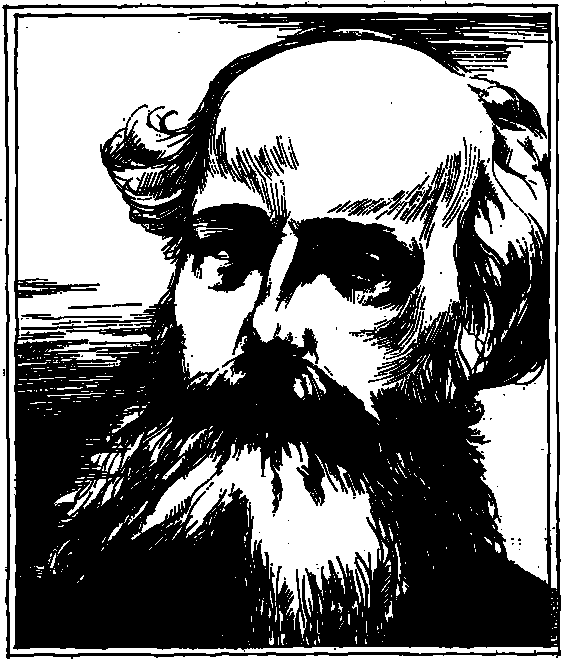
\includegraphics[width=0.8\textwidth]{figures/maxwell.pdf}
\end{center}
{\small \textsf{{James Clerk Maxwell [1831-1879]}} -- \textsf{\footnotesize famed Scottish physicist; he was the founder of theoretical electrodynamics. Maxwell's equations describe the behaviour of electromagnetic waves and an electromagnetic field regardless of its origin. Maxwell is the author of the electromagnetic theory of light. The theoretical value of the velocity of light follows automatically from his equation. Maxwell's theory is the basis for the relationship between the permittivity and the refractive index, the orthogonality of the electric and magnetic vectors in a wave, and the existence of light pressure. Of no less importance was Maxwell's contribution to the kinetic theory of gases. Maxwell worked out the velocity distribution law for gas molecules.}}



Maxwell's laws belong to the fundamental general laws of nature. They are not derived by logical reasoning and mathematical calculations. Fundamental laws of nature are generalizations of our knowledge. Laws of nature are discovered, found or ascertained. It is a matter of great interest to historians of science and to psychologists to follow out the chain of guesses and creative perception by means of which a genius discovers a law of nature. This, however, is a subject for a special book.

As for the reader and myself, nothing is left but to analyze a certain outline of consecutive assumptions that lead to Maxwell's laws.

What was known to Maxwell when he set himself the task of expressing in concise symbolic form the laws governing the behaviour of electric and magnetic fields? In the first place, he knew that any point in space in the vicinity of an electric charge can be specified by a vector of electric force (intensity), and any point near an electric current, by a vector of magnetic force.

But are stationary electric charges the only source of an electric field? And are electric currents the only source of a magnetic field?

Maxwell answered these questions in the negative and proceeded in his search for the laws of an electromagnetic field along the following series of guesses.

Faraday showed that an electric current is induced in a wire loop which is threaded by an alternating flux of magnetic lines of force. But a current is produced when an electric force acts on electric charges. This being so, we can express Faraday's law by the following phrase: an electric field is set up in a wire loop through which an alternating magnetic flux passes.

But is it essential that the magnetic flux is encompassed by a wire loop? Is it not all the same to the electric field where it is set up: in a metal conductor or in empty space? Let us assume that it is all the same. Then the following statement is valid: a closed electric line of force appears near a variable flux of magnetic lines of force.

Thus the first two of Maxwell's laws concerning an electric field have been formulated. We contend that an electric field is set up in two ways: by electric charges (in which case the lines of force start at positive and end at negative charges) and by a variable magnetic field (in which case the electric line of force is closed and encompasses the variable magnetic flux).


Next we attempt to find the laws concerning a magnetic field. A magnetic field is set up by currents; this Maxwell knew. Direct (constant) current is the source of a constant magnetic field, and alternating (variable) current sets up a variable magnetic field. But we know that an alternating current is produced in wire by a variable electric field. And what if there is no wire, but only a variable electric field existing in empty space? Is it not logical to assume that a closed magnetic line of force is produced near a variable flux of electric lines of force? Its symmetry makes this picture very attractive: a variable magnetic flux sets up an electric field, and a variable electric flux, a magnetic field.

Thus, the two laws concerning electric fields are supplemented by two more that govern the behaviour of magnetic fields. That a magnetic field has no sources (there being no magnetic charges) is the third law, and that a magnetic field is produced by electric currents and a variable electric field is the fourth law.

Maxwell's four laws can be written with exceptional elegance in the form of mathematical equations. With respect to them and quoting a line from Goethe, the great Austrian physicist Ludwig Eduard Boltzmann (1844-1906) wrote: ``Was it a god who wrote these lines \ldots'' Unfortunately, I cannot acquaint the reader with the meaning expressed by these equations. This would require from him a knowledge of mathematics at a level above that used in this series (\figr{fig-5.1}).

\begin{figure}[!ht]
\centering
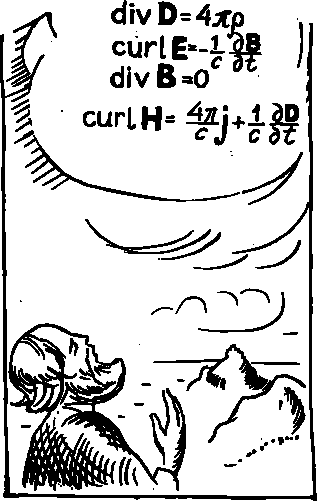
\includegraphics[width=0.4\textwidth]{figures/fig-05-01.pdf}
\caption{The four equations of Maxwell.}
\label{fig-5.1}
\end{figure}


Maxwell's laws indicate that a variable magnetic field cannot exist without an electric field, and a variable electric field, without a magnetic field. This is why the two adjectives, electric and magnetic, are not separated by a comma. An electromagnetic field is a single entity.

As we move away from the charges that are the sources of an electromagnetic field, we deal with electromagnetic matter, so to speak, in the pure form. It is not necessary to consider pencils of lines of force. Maxwell's laws can be written so that they are applicable to a point in space. Then they sound especially simple: at a point where the electric vector varies with time, there exists a magnetic field vector that also varies with time. 

``But is not all the aforesaid pure imagination?'' asks the reader. In practice, as a matter of fact, it is absolutely impossible to measure the magnitudes of rapidly varying electric and magnetic field vectors at a point in space.

True! But the grandeur of laws of nature is assessed by the consequences that follow from them. The consequences, in this case, are legion. It is no exaggeration whatsoever to contend that all of electrical and radio engineering is contained in Maxwell's laws.

It is imperative, however, to tell about one vital conclusion based on Maxwell's equations. It can be shown by faultlessly rigorous calculations that electromagnetic radiation must exist.

Assume that there are charges and currents in some bounded region of space. Various energy transformations may occur in this system. Mechanical or chemical sources produce electric currents, and the currents, in their turn, drive mechanisms and evolve heat that is liberated by the wires. Now let us calculate all the debits and credits. But they do not tally! The calculations show that some fraction of the energy of our system has escaped into space.

Has theory anything to say about this ``radiated'' energy? It seems that it has. The solution of the necessary equation is of quite complex form near the source, but at distances substantially exceeding the size of the ``radiating'' system, the picture becomes highly clear-cut and, what is most important, lends itself to experimental proof.

At great distances electromagnetic radiation, as we call the energy deficiency in our system of moving charges, can be characterized at each point in space by its direction of propagation. In this direction the electromagnetic energy travels at a velocity of about \SI{300000}{\kilo\meter\per\second}. This figure follows from the theory! The second conclusion of the theory is that the electric and magnetic vectors are perpendicular to the direction of wave propagation and perpendicular to each other. Thirdly, the intensity of electromagnetic radiation (energy per unit area) decreases inversely proportional to the square of the distance.

Since it was known that light travels with about the same velocity that had been calculated for electromagnetic radiation, and sufficiently complete information on the polarization of light had been acquired to indicate that luminous energy has some ``transverse'' properties, Maxwell came to the conclusion that light is a form of electromagnetic radiation.

Ten years after Maxwell's death, at the end of the eighties, the famous German physicist Heinrich Rudolf Hertz (1857-1894) experimentally substantiated all the conclusions from Maxwell's theory. Following these experiments, Maxwell's laws and their equations were firmly established forever and ever as one of the few cornerstones supporting the structure of modern physics.

\section{Mechanical Models of Radiation}
Mechanical models are contrasted with mathematical models. Mechanical models can be contrived by using balls, springs, strings, rubber cords, etc. A mechanical model helps to make some phenomenon visual. By building a mechanical model and demonstrating its operation we help a person to understand the phenomenon by saying: ``Such and such a quantity behaves similar to such and such a displacement.'' Far from all mathematical models can be contrasted with a mechanical one.

Before we take up electromagnetic radiation, a fact established by innumerable experiments and following by strict logic from Maxwell's equations, we should discuss the feasible mechanical models that can be contrived for radiation.
There are two such models: corpuscular and wave. We can make a toy which ``radiates'' streams of tiny particles -- peas or poppyseed -- in all directions. This is the \emph{corpuscular model} because the word ``corpuscle'' means a particle.

A particle flying at a certain velocity and having a certain mass should conform to the laws of mechanics. Particles are capable of colliding, changing their directions of motion, but only if the collision obeys the laws of conservation of energy and momentum. Some bodies may prove impenetrable to the particles. In such cases the particles must bounce off the bodies according to the law: the angle of incidence equals the angle of reflection. Particles can be absorbed by the medium. 

If particles can travel easier in one medium than in another, we can readily explain refraction. After passing through a hole in an opaque screen, a stream of particles emerging from a point source should travel within a cone. True, a small amount of scatter is possible because a small fraction of the particles are reflected by the edges of the hole. Of course, these reflected particles can only be chaotic and cannot produce any regular pattern that extends outside the geometric shadow.


The \emph{wave model} is usually demonstrated by a water bath. The water can easily be made to oscillate at some point. From this point, as from a stone dropped into water, concentric waves spread outward in ever-widening circles. We can see the wave-like surface of the water. Energy is propagated in all directions and a wooden chip, floating at some distance, begins to oscillate with the frequency of the point to which we supply energy.

Sound vibrations are somewhat more difficult to see. But we can conduct absolutely convincing experiments to show that sound is transmitted by the mechanical displacement of the medium from point to point.

A great many phenomena are equally well explained by both the wave and corpuscular models. Both models are equally suitable, however, only when an additional condition is complied with: a wave acts just like a stream of particles if the obstacles and holes it encounters are much smaller than the wavelength.

As we can readily calculate from the main formula, used to describe the wave model, $c = \nu \lambda$, the average frequency of a human voice of \SI{1000}{\hertz} corresponds to a wavelength of \SI{30}{\centi\meter}. Such a wave can go around a corner if it has to pass through holes one metre in size. But if the hole has a size of the order of one centimetre, we can contend that a sound beam passes through it only when a straight line connecting the source and receiver of the sound meets no obstacles.

Suppose that a radio set is speaking in a room with open windows high up on the wall. A man sitting outside on a bench under the window can hear what is going on. If the windows are tightly closed and the walls are thick, the sound can pass only through the keyhole of the door. Now, even the most sensitive detector receives a signal only if the source of the sound, the keyhole and the detector are on a straight line. Here sound energy is transmitted like a stream of particles.

It can readily be shown by both reasoning and experiments in a water bath that the law of reflection from a wall of a roughness less than the wavelength is complied with by the wave model as well.

The reader knows quite well how sound or any other wave is reflected by a smooth plane surface. Interesting problems may be posed when the reflecting surface is of curved shape.

One such problem follows. What kind of surface is required to collect a wave, emitted by a point source, back into a single point? The shape of this surface must be such that rays from one point, incident to the surface at various angles, are all reflected to another single point. What is this surface?

The reader may recall one remarkable property of the curve called an ellipse. The distance from one focus of the ellipse to any point of the curve plus the distance from this point to the other focus is the same for all points on the ellipse. Now imagine that the ellipse is rotated about its major axis. The rotating curve describes a surface which is said to be an ellipsoid. (Its shape resembles a symmetrical egg.) Another property of an ellipse is the following. If an angle is drawn with its vertex at a point of the ellipse~and its sides passing through the foci, the bisector of this angle is normal to the ellipse at the point. This means that if a wave or a stream of corpuscles is emitted at one focus of the ellipsoid, it is reflected by the internal surface and arrives complete only at the other focus.

As far as sound waves are concerned, the walls and ceiling are sufficiently smooth. If the ceiling is vaulted, a special case of sound reflection can be observed. Since the shape of the arched ceiling is close to that of an ellipsoidal surface, sound emitted at one focus is reflected by the ceiling to the other focus. This property of vaulted ceilings was known in ancient times. In the Middle Ages, during the inquisition, it was made use of to eavesdrop. Two persons, disclosing their thoughts to each other in a quiet voice had no idea that they were being overheard by the dozy monk sitting at the other end of the tavern (\figr{fig-5.2}).

\begin{figure}[!ht]
\centering
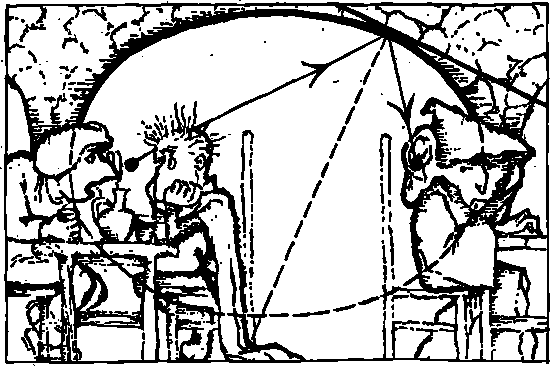
\includegraphics[width=\textwidth]{figures/fig-05-02.pdf}
\caption{Reflection from an ellipsoidal shape.}
\label{fig-5.2}
\end{figure}

The corpuscular and wave models are equally suitable to explain this phenomenon. But a phenomenon like the collision of billiard balls cannot be explained by the wave model.

There are, on the other hand, several vital facts that the corpuscular model cannot cope with.

Primarily, this concerns \emph{interference}, i.e. a summation in which the sum may turn out to be less than the addends or even equal to zero. If two waves arrive at a point and are added together, of prime importance is their difference in phase at this point. If the crest of one wave coincides with the crest of the other, the waves add up. But if the crest of one wave coincides with the trough of the other and their amplitudes are the same, addition has a zero result. 

The waves arriving at a single point cancel out each other. Then two wave fields are superimposed, at certain places the waves are added together and at others they are subtracted one from the other. This is interference. This is the first phenomenon that is absolutely impossible to deal with using the language of streams of particles. If radiation behaves like a stream of peas, then the superimposed fields must intensify each other at all places and at all times.

The second important phenomenon is \emph{diffraction}, i.e. bending around corners, or passing around obstacles. A stream of particles cannot act in this way, but a wave must behave in exactly this way. In school, diffraction is demonstrated by generating waves in a small bath of water. Then a partition with a hole is put into the path of the waves and the bending around corners becomes visible to the naked eye. The cause of this phenomenon is entirely natural. The particles of water begin to vibrate in the plane of the hole. Each point lying in the plane of the hole produces a wave, all the points having the same rights as the initial source of radiation. Nothing hinders this secondary wave from ``bending around a corner''.

Interference and diffraction can be demonstrated without difficulty if the condition mentioned above is complied with: the wavelength must be greater than or at least commensurable with the size of the obstacles or holes. We shall refine this condition and deal with diffraction and interference in more detail in Book~4.
Next we shall discuss the change in the frequency of waves observed when the source of radiation is in motion. That this phenomenon is a necessary consequence of the wave model was shown by the Austrian physicist Christian Johann Doppler (1803-1853) in the early days of theoretical physics.

We shall derive the equation of the \emph{Doppler effect}, as it is called; it shall prove useful later. Assume, for the sake of clearer representation, that an automobile is approaching a marching brass band. The number of periodic compressions of the air reaching the driver's ear per unit time is greater, than if the automobile were at rest, by the ratio $(c+u)/u$, where $c$ is the velocity of propagation of the waves and $u$ is the relative velocity of the source of the waves and their detector (the driver in our case). Hence
\begin{equation*}%
\nu' = \nu \left( 1 + \frac{u}{c} \right)
\end{equation*}
This means that the heard frequency $\nu'$ is higher when the automobile and band approach each other (the pitch is higher when $u > 0$) and drops when they are moving away from each other (the pitch is lower and $u<0$). Getting a little ahead of our story, we can say that for light waves this conclusion is the following: a ``red shift'' occurs when the source is receding. The reader will appreciate the importance of this conclusion when we discuss the observation of the spectra of distant stars.

From a long time in the past and down to the twenties of our century, philosophers and scientists have often argued whether some case of energy transmission is of a wave or a corpuscular nature. Experiments indicated that any kind of radiation has two aspects. Only a combination of these two aspects properly represents reality. Theory has elevated this fact to the rank of a principal law of nature. Wave mechanics, quantum mechanics and quantum physics are equivalent names for the modern theory describing the behaviour of fields and particles.


\section{Two Aspects of an Electromagnetic Field}

In certain phenomena electromagnetic radiation behaves like waves and in others like a stream of particles. In this sense, Maxwell's laws are prone to ``error''; they only outline the wave aspect of electromagnetic radiation.


In complete agreement with experimental investigations, a solution of Maxwell's equations leads to the conclusion that we can always conceive of electromagnetic radiation as being the sum of waves of various lengths and intensities. If the radiating system is an electric current of fixed frequency, the radiation consists of a ``monochromatic'' (single-colour) wave.


An electromagnetic wave is illustrated in \figr{fig-5.3}. To understand the changes that take place in space in the transmission of electromagnetic energy, we must ``pull'' our figure as a rigid whole along the axis of abscissas. This picture is obtained as a solution to Maxwell's equations. It is what enables us to speak of electromagnetic waves. In employing this term and in resorting to the analogy between an electromagnetic wave and one spreading outward in water when we drop a stone, we must proceed with extreme caution. Pictorial representations can easily mislead us. A wave on water is only a model of an electromagnetic wave. This means that electromagnetic waves and waves on water behave the same only in certain respects.

\begin{figure}[!ht]
\centering
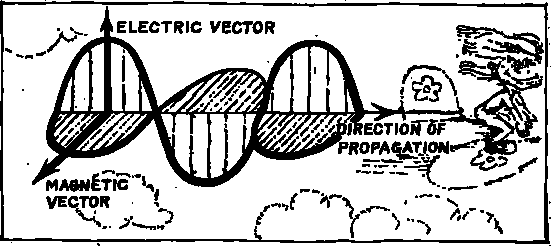
\includegraphics[width=\textwidth]{figures/fig-05-03.pdf}
\caption{A visualisation of the electromagnetic wave.}
\label{fig-5.3}
\end{figure}

But are not \figr{fig-5.3}, illustrating an electromagnetic wave, and a water wave, which alternately raises and lowers a wooden chip thrown into the sea, alike as two peas? Nothing of the kind! Consider carefully the essence of the drawing. Plotted along the vertical axis are the electric field vectors and not some kind of spatial displacements!

The magnitude of the ordinate at each point indicates the force that an electric charge would be subject to if it were placed at that point. Strictly speaking, nothing is moved from its place during the travel of an electromagnetic wave. It is absolutely impossible in practice to conduct an experiment showing the variation in value of an electromagnetic wave at some point, even for very slow vibrations.

Hence, the concept of an electromagnetic wave is of a theoretical nature. We confidently speak of the existence of electromagnetic waves because we listen to the radio. We have no doubt that an electromagnetic wave has a certain frequency because we must tune our radio set to a definite frequency for the reception of a definite broadcasting station. We are sure that the concept of length is applicable to an electromagnetic wave. Not only can we measure the wave velocity and calculate the wavelength by formula $c = \nu \lambda$, which relates the frequency, wavelength and velocity of propagation, but we can obtain an idea of the length of electromagnetic waves from diffraction, i.e, bending around a corner or an obstacle. The principle involved in this last kind of measurement is the same as for waves travelling on water.

It is absolutely necessary to warn the reader that he should not attempt to work out a visualizable conception of an electromagnetic wave because, as mentioned at the beginning of this section, electromagnetic radiation not only ``resembles'' waves, but in many cases ``reminds'' us of the behaviour of a stream of particles. To try to imagine something that simultaneously resembles a stream of particles and a wave is entirely contrary to reason. 

We are discussing physical processes that cannot be represented by chalk on a blackboard. This does not imply, of course, that we cannot obtain exhaustive knowledge of an electromagnetic field. We must keep in mind that graphic pictures are only a teaching aid, a method for more easily memorizing symbols. But we should not forget that the wave picture is only a model of electromagnetic radiation, and nothing more! Where feasible, we employ this model, but we should not be surprised that this model can only lead us into error in some cases.

In exactly the same way, the corpuscular aspect of an electromagnetic field is not always observed. It would, of course, be simpler if the conditions under which these two aspects are manifested were mutually exclusive. But no, this is not so. Even in describing one and the same experiment, it is often necessary to speak in two languages.

It is nevertheless simpler (or, it is better to say, it previously was simpler) to observe the corpuscular aspect of electromagnetic radiation for short waves. In an ionization chamber and other similar instruments, we can observe the collision of particles of electromagnetic radiation with an electron or other ``honest'' particles. The collision may resemble that of billiard balls. It is absolutely impossible to understand such behaviour if we only resort to the wave aspect of electromagnetic radiation.

Using the language of Maxwell's theory, let us consider the production of electromagnetic radiation. A system of charges oscillates with a certain frequency. The electromagnetic field varies in time with these oscillations. The frequency $\nu$ of oscillations of the field divided by the velocity of propagation (\SI{300000}{\kilo\meter\per\second}) gives the wavelength of the radiation.

When we deal with the same phenomenon in the language of quantum physics, it is described as follows. We have a system of charges characterized by a system of discrete energy levels. For some reason the system got into an excited energy state, but did not exist long in this state and went over to a lower energy level. The energy $E_{2}-E_{1}=h\nu$ evolved in this transition is radiated in the form of particles called photons. We are already acquainted with constant $h$ (see page~\pageref{ang-mom}). It is Planck's constant.



If the energy levels of the system are very close together, the photon has low energy, low frequency and, consequently, a long wavelength. Here the quantum corpuscular aspect of the electromagnetic field is hardly noticeable and manifests itself only in absorption phenomena, which are associated with extremely small changes in the energy of electrons or atomic nuclei (magnetic resonance). In the case of waves of long length we do not succeed in observing collisions of a photon with particles, like the collisions of billiard balls.

We shall briefly mention facts that, so to speak, drove physicists into a corner, forcing them to agree that wave theory (which they had believed in for many years as the complete and comprehensive truth) is incapable of explaining all the facts concerning electromagnetic fields. There are many such facts but, for the time being, we shall restrict ourselves to a phenomenon called the photoelectric effect. After the reader has consented that a comprehensive picture of the electromagnetic field cannot be created without its corpuscular aspect, we shall discuss Hertz's wonderful experiments on which all of radio engineering is based. We shall show how the wave aspect of the electromagnetic field was depicted, not only in its general form, but in all its details as well.

\section{Photoelectric Effect}

The fine sonorous name ``photon'' appeared on the scene somewhat later than the product of Planck's constant $h$ by the frequency $\nu$ of an electromagnetic wave. As mentioned above, the transition of a system from one energy state to another is accompanied by the absorption or emission of a portion of energy equal to $h\nu$. The first to come to this conclusion, at the turn of the century, was the famous German physicist Max Karl Ernst Ludwig Planck (1858-1947). He showed that this was the only way that the radiation of incandescent bodies could be explained. 

The argument concerned electromagnetic waves produced by a method having nothing in common with radio engineering. It had not yet been proved at that time and was not recognized by all physicists that what is valid for light is true for radio waves as well. This was the situation even though Maxwell's laws definitely proved that there is no difference in principle between radio waves and any other electromagnetic waves, including light. An understanding and the experimental proof of the universal validity of Planck's statement came later.


Planck's work concerned the radiation of light in discrete portions, i.e. in \emph{quanta}. The work did not note, however, that the quantum nature of radiation made it inevitable to introduce the corpuscular aspect of the electromagnetic field into the discussion. A field was said, at that time, to radiate in portions, but a portion was thought to be a certain wave train.

The most important step, i.e. the recognition of the fact that the radiated portion of energy $h\nu$ is the energy of a particle which was immediately named the photon, was made by Einstein. He showed that only corpuscular concepts could explain the \emph{photoelectric effect (photo-effect)}, i.e, the ejection of electrons from solids under the influence of light.

Shown schematically in \figr{fig-5.4} is the apparatus employed at the end of last century to begin a detailed study of the phenomenon called the \emph{extrinsic photoelectric effect}.

\begin{figure}[!ht]
\centering
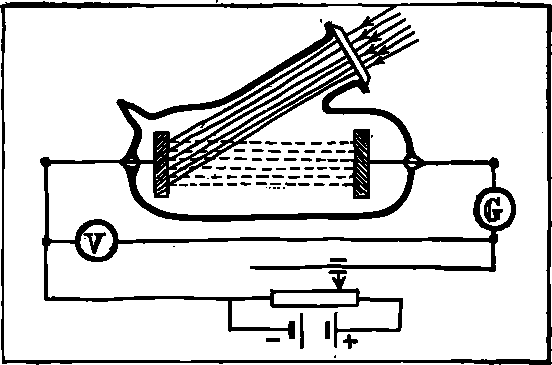
\includegraphics[width=\textwidth]{figures/fig-05-04.pdf}
\caption{The schematic drawing for studying the photoelectric effect.}
\label{fig-5.4}
\end{figure}

In 1888, Heinrich Hertz reported that light in some way affects the electrodes of a vacuum tube. He was evidently the first to notice this phenomenon. Working at about the same time, the Swedish chemist Svant\'e August Arrhenius (1859-1927), the German physicist Wilhelm Ludwig Franz Hallwachs (1859-1922), the Italian physicist Augusto Righi (1850-1921) and the outstanding Russian physicist Alexander Grigoryevich Stoletov (1839-1896) showed that illumination of the cathode produces an electric current. If no voltage is applied across the tube shown in \figr{fig-5.4} (it is called a \emph{photoelectric cell}), only a negligible part of the electrons, ejected from the cathode through the impact of light, reach the opposite electrode. A weak accelerating voltage (with a negative photocathode) increases the current. Finally, as the voltage is increased, the current reaches its saturation value: all the electrons (whose number is quite definite at the given temperature) reach the anode.

The magnitude of the photocurrent is strictly proportional to the light intensity. The light intensity is uniquely determined by the number of photons. It immediately occurs to us (and this is confirmed by rigorous calculations and experiments) that each electron is ejected by one photon.

The energy of the photon is expended in liberating an electron from the metal and imparting a velocity to it. This is expressed by an equation first derived by Albert Einstein in 1905. Here it is:
\begin{equation*}%
h \nu = \frac{mv^{2}}{2} + A
\end{equation*}
where $A$ is the work function (see page~\pageref{work-func}).

The energy of the photon must at least exceed the work function, i.e. the minimum energy it is necessary to expend to eject an electron from the metal. This means that for the photon each energy (and the energy is uniquely related to the ``chromaticity'') has its threshold value of the photoelectric effect.

Photoelectric cells, based on the extrinsic photoeffect, are extensively used in photorelays, television and sound motion pictures.

The sensitivity of a photoelectric cell can be increased by filling it with gas. Here the current is increased because the liberated electrons break up the neutral molecules of gas and unite them with the photocurrent.

The photoelectric effect, true, not the one we have described, but the so-called \emph{internal photoelectric effect}, occurring at the boundary of the \emph{p-n} layer in semiconductors, is of exceptional importance in modern engineering. To avoid interrupting our discussion, however, we shall postpone the treatment of the application of the photoelectric effect until Book~4. Here we mentioned this phenomenon only to demonstrate the inevitability of recognizing that an electromagnetic field has corpuscular properties.

For many years photons were the forlorn stepsons of physics. Proof of the existence of photons and the investigation of the laws of the photoelectric effect anticipated the founding of quantum physics by about 20 to 30 years. Only by the end of the twenties, when these laws had been established, it became clear why the same numerical constant, Planck's constant $h$, appears both in the formula for the energy of a photon and in the formula, discussed on page~\pageref{ang-mom}, that determines the possible values of the angular momentum of particles.


The value of this constant is determined from many different kinds of experiments. The photoelectric effect, the Compton effect (change in the wavelength of $X$-rays in scattering), the radiation produced upon the annihilation of particles and many other experiments yield the same numerical value.


\section{Hertz's Experiments}

Now let us consider the way in which the hypotheses concerning the wave aspect of the electromagnetic field were proved.

Logic and mathematics extract many consequences from Maxwell's laws. These consequences may turn out to be valid or they may not be confirmed by experiments. A physical theory becomes a part of science only after being experimentally checked. The establishment of electromagnetic field theory -- from separate facts to a general hypothesis, from the hypothesis to the consequences and to the final stage, an experiment that provides decisive proof -- is the only proper procedure for a naturalist. This highway to scientific truth is especially defined in the case of the laws of the electromagnetic field.

For this reason we shall discuss Hertz's experiments in more detail. They are still being used by teachers and lecturers to demonstrate to students of schools and institutes how a scientist gains confidence in the validity of laws of nature.
\begin{figure}[!ht]
\centering
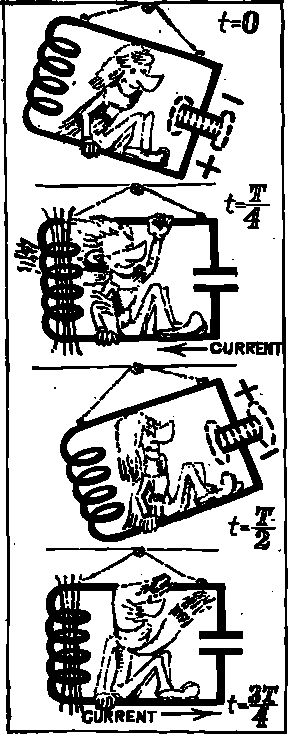
\includegraphics[width=0.4\textwidth]{figures/fig-05-05.pdf}
\caption{An oscillatory circuit.}
\label{fig-5.5}
\end{figure}

We must begin our story in 1853, when the famous British physicist Lord Kelvin proved mathematically that electric oscillations occur when a capacitor is discharged through an inductance: the charge on the capacitor plates, the voltage at any point in the circuit and the current all vary according to the law of harmonic oscillations. If we assume that the resistance of the circuit is negligible, these oscillations will continue forever.

The pictures in \figr{fig-5.5} demonstrate the phenomena that occur in a so-called \emph{oscillatory circuit}. At the initial instant of time the capacitor is charged. Current flows as soon as the circuit is closed. After one-fourth of a period, the capacitor is completely discharged. Its energy, $q^{2}/2C$, is converted into the energy of the coil's magnetic field. The current is at a maximum at this instant. 

Continuing in the same direction, the current gradually decreases. After a half-period, the current drops to zero, the magnetic energy, $LI^{2}/2$, disappears, the capacitor is completely charged again and its energy is restored. But the sign of the voltage is reversed. Then the process is repeated in the reverse direction. After a certain time $T$ (the period of oscillation), everything returns to the initial state and the process begins again.

Electric oscillations would continue to infinity except for the inevitable resistance to current flow. Energy is lost in each period due to resistance. As a result, the oscillations decrease in amplitude and are soon damped.

The obvious analogy with a load suspended by a spring enables us to dispense with an algebraic analysis of the process and to reason out the period of oscillations of such a circuit. (The reader should refresh his memory of the corresponding pages in Book~1.) It is sufficiently evident, as a matter of fact, that the electric energy
of the capacitor is equivalent to the potential energy of the compressed spring, and the magnetic energy of the coil, to the kinetic energy of the weight.

Associating analogical quantities, we ``derive'' the formula for the period of oscillations occurring in the circuit: $q^{2}/2C$ is the analogue of $kx^{2}/2$, $LI^{2}/2$ of $mv^{2}/2$, $k$ of $1/C$ and $L$ of $m$. Hence the frequency of oscillations is 
\begin{equation*}%
\nu = \frac{1}{2\pi} \sqrt{LC}
\end{equation*}
because the corresponding formula for mechanical oscillations is of the form
\begin{equation*}%
\nu = \frac{1}{2\pi} \sqrt{\frac{k}{m}}
\end{equation*}
Now let us try to guess the train of thought of Hertz, who made it his aim to prove the existence, without leaving his laboratory, of electromagnetic waves propagating at a velocity of \SI{300000}{\kilo\meter\per\second}. For this purpose, an electromagnetic wave is required with a wavelength of the order of \SI{10}{\meter}. If Maxwell was right, the electric and magnetic vectors should oscillate with a frequency of \SI{3d8}{\hertz}; pardon me, cycles per second. At that time Hertz did not know that his name would be perpetuated as the unit of frequency.

\begin{figure}[!ht]
\centering
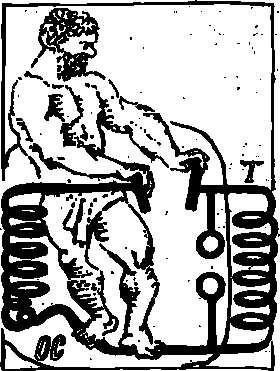
\includegraphics[width=0.4\textwidth]{figures/fig-05-06.pdf}
\caption{An oscillator circuit for detecting and producing electromagnetic waves.}
\label{fig-5.6}
\end{figure}

``What shall I begin with?'' he probably asked himself. In the first place, since the oscillations are damped, it is necessary to devise an arrangement that recommences the process when the current stops. This is not a difficult task. The required circuit is illustrated in \figr{fig-5.6}. An alternating voltage is applied across the primary winding of transformer $T$. As soon as it reaches the breakdown voltage between the metal spheres connected to the secondary winding, a spark is initiated. This spark is what closes the oscillatory circuit $OC$, acting like a switch key, and dozens of oscillations, with a decreasing amplitude and a more or less high frequency, pass through the circuit.

But a high frequency is required. What can be done to obtain one? We can reduce the self-induction and the capacitance. But how? We replace the coil by a straight wire, and we spread the capacitor plates apart and reduce their area. Into what does the oscillatory circuit degenerate? It is converted into two simple rods ending in metal spheres between which sparks jump.


%\newpage

\begin{center}
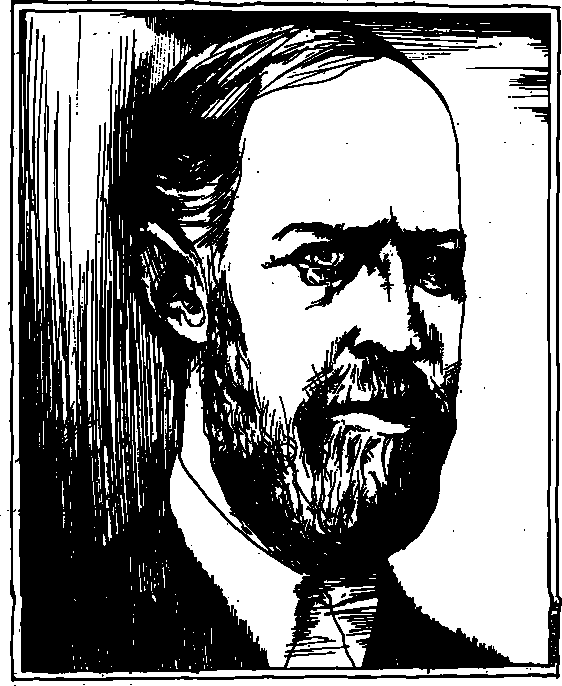
\includegraphics[width=0.8\textwidth]{figures/hertz.pdf}
\end{center}
{\small \textsf{{Heinrich Rudolph Hertz [1857-1894]}} -- \textsf{\footnotesize brilliant German physicist; using his ``oscillator'' and ``resonator'' he proved in experiments that an oscillatory discharge produces electromagnetic waves in space. Hertz showed that electromagnetic waves are reflected, refracted and subject to interference, thereby confirming Maxwell's theory. Hertz's experiments laid the foundation of radio engineering. In his first radio broadcast in 1895, Alexander Stepanovich Popov, inventor of the radio, transmitted two words: ``Heinrich Hertz''.}}

Thus Hertz got the idea for his oscillator which can serve both as a source and as a detector of electromagnetic waves.

It was difficult for Hertz to predict beforehand the inductance and capacitance of this unusual ``circuit'' of which almost nothing remained. The inductance and capacitance of the oscillator are not concentrated in some definite place in the circuit but are distributed along the rods. Some other theory is required.

A discussion of this new approach to electric circuits with currents of very high frequency would take us too far from our main subject. The reader can believe our word that oscillations of high-frequency current really do occur in Hertz's oscillator.

The ``transmitter'' and ``receiver'' of waves, used by Hertz, were practically the same. In the ``transmitter'' the waves were produced by sparks periodically jumping the gap between the spheres in accordance with the operation of the transformer that applied voltage to the oscillator. The width of the spark gap could be regulated by a micrometric screw. Serving as the receiver, or detector, was either a rectangular turn of wire interrupted by a spark gap or two small rods that could be adjusted as required to obtain a gap within a fraction of a millimetre.

In his first work, published in 1885, Hertz showed that oscillations of extremely high frequency can be obtained by the above-described method and that these oscillations actually do set up an alternating field in adjacent space. The existence of this field, he wrote, can be demonstrated by sparks jumping across a gap in the ``receiver''. Hertz called this receiving oscillator a resonator. He immediately grasped the principle of detecting an electromagnetic field. This principle is the basis of modern radio engineering.

Incidentally, we may note that neither in Hertz's works nor in others published in the next few decades do we find the terms ``electromagnetic waves'' or ``radio waves''. They speak only of electric waves or of waves of electrodynamic force.
In his next work Hertz showed that, in accordance with the requirements of Maxwell's theory, the dielectric medium (a bar of sulphur or paraffin) affects the frequency of the electromagnetic field. When he received this article, Helmholtz, the editor of the scientific journal, sent Hertz a postcard with the message: ``Your manuscript has been received. Bravo! I shall send it to the press on Thursday.''

Hertz's work in which he showed that electromagnetic waves can be reflected made a tremendous impression on the physicists of his day. The waves were reflected by a zinc screen, $4 \times \SI{2}{\meter}$ in size. The oscillator was \SI{13}{\meter} from the screen and at a height of \SI{2.5}{\meter} above the floor. The tuned resonator was arranged at the same height and could he moved between the oscillator and screen. Setting the resonator at various distances from the screen and observing the intensity of the sparks, Hertz established that there were maximums and minimums typical of the interference phenomena that set up standing waves. The wavelength was found to be approximately \SI{9.6}{\meter}.

I should like to emphasize the fact that at that time no one could say what material could serve as a mirror for electromagnetic waves. Today we know that waves of such length do not penetrate metals, but are reflected from them.

In trying to obtain additional proof of Maxwell's theory, Hertz reduced the geometrical size of his apparatus until he reached a wavelength of \SI{60}{\centi\meter}. In 1888 he published the work \emph{On the Beams of Electric Force}. He was able to concentrate electromagnetic energy by means of parabolic mirrors. The rods of the oscillator and resonator were arranged at the foci of the mirrors. Employing the mirror-type transmitter and receiver, Hertz showed that electromagnetic waves do not pass through metals, but wooden screens do not check them.
\begin{figure}[!ht]
\centering
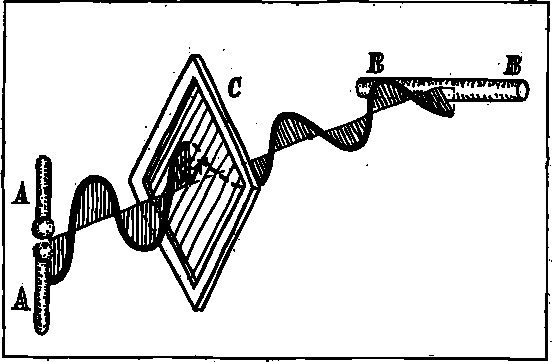
\includegraphics[width=\textwidth]{figures/fig-05-07.pdf}
\caption{A demonstration of the polarization of electromagnetic waves.}
\label{fig-5.7}
\end{figure}


\figr{fig-5.7} shows how Hertz demonstrated the polarization of electromagnetic waves. He arranged grating $C$, made of parallel copper wires, in the path of the electromagnetic beam produced by oscillator $AA$ . Hertz showed that when he turned the grating, the intensity of the spark in resonator $BB$ was varied. When the grating wires were parallel to the electric vector and perpendicular to the axes of the oscillators, the beam did not pass through the grating. Thus, the transverse character of an electromagnetic wave was proved.

Finally, to study the refraction of the waves, Hertz made a prism weighing over one tonne from an asphalt compound. The refractive index of the asphalt for waves \SI{60}{\centi\meter} in length could he measured with high accuracy. It was found to equal 1.69.

The proof of the existence of electromagnetic waves, measurement of their length, and the establishment of the laws of their reflection, refraction and polarization are all the results of only three years of research! Truly a capacity for work to be admired.

 
\section{Classification of Electromagnetic Radiation}

Physicists deal with electromagnetic radiation over a huge range. The electromagnetic radiation of current of city mains frequency is absolutely negligible. Practically, the feasibility of detecting electromagnetic radiation begins with frequencies of the order of dozens of kilohertzes, i.e. at wavelengths equal to hundreds of kilometres. The shortest waves have a length of the order of ten thousandths of a micron, i.e. a frequency of the order of a thousand million gigahertzes.

\emph{Radio waves} are in the range of electromagnetic radiation produced by electrical engineering means, i.e. as a result of the oscillation of electric currents. The shortest radio waves have a wavelength of hundredths of a millimetre.

Beginning with several hundred microns and smaller is the wavelength range of radiation due to energy transitions inside molecules, atoms and atomic nuclei. As we can see, this range substantially overlaps the radio range.

Visible light occupies a narrow range. Its limits are 0.38 to 0.74 micron. Radiation of longer wavelength, not obtained by radio engineering techniques, is said to be \emph{infrared}; that of shorter wavelength is called \emph{ultra-violet} and extends down to a wavelength of about 0.1 micron.

Electromagnetic radiation produced in X-ray tubes overlaps the range of ultraviolet waves and extends down to a wavelength of 0.01 micron, where it overlaps the gamma ray range. \emph{Gamma rays} are produced in nuclear decay, in nuclear reactions and in collisions between elementary particles.

\begin{figure}[!ht]
\centering
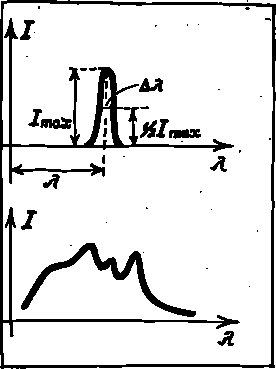
\includegraphics[width=0.4\textwidth]{figures/fig-05-08.pdf}
\caption{Intensity curves of monochromatic radiation. Top: single monochromatic radiation. Bottom: overlapping monochromatic radiations.}
\label{fig-5.8}
\end{figure}

The principal characteristic of any electromagnetic radiation is its spectrum. The spectrum is a graph on which the intensity (i.e. the energy per unit time per unit area) is plotted in the vertical direction and the wavelength or frequency in the horizontal direction. The simplest spectrum is that of monochromatic (``single-colour'') radiation. Its graph consists of a single line of extremely narrow width (\figr{fig-5.8}, above). The degree of monochromaticity of the line is specified by the ratio $\lambda/\Delta \lambda$. A broadcasting station produces almost purely monochromatic radiation. For a short-wave station, for instance, operating in the \SI{30}{\meter} range, $\lambda/\Delta \lambda$ equals about 1000.

Excited atoms, for example, atoms of gases in daylight lamps (the excitation being due to the collisions of positively and negatively charged particles travelling toward the anode and cathode), produce a spectrum consisting of a great number of monochromatic lines with a relative width of $1/100000$. Lines are observed in magnetic resonance with a relative width as small as \num{d-7}.


Strictly speaking, no continuous spectra exist. However, if the lines overlap, the experiment yields an intensity curve of the kind shown below in the same illustration.

Information on an electromagnetic spectrum can be obtained either by investigating radiation or by studying absorption. In general, both experiments provide the same information. This is evident from the principal law of quantum physics. In radiation, the transition of the system is from a higher to a lower energy level; in absorption, it is from a lower to a higher level. But the difference in energy, which determines the frequency of radiation or absorption, is exactly the same. Which spectrum we investigate, radiation or absorption, is, simply a matter of convenience.

In characterizing a radiation spectrum, we can, of course, use either wave or corpuscular terminology. Employing the wave aspect of radiation, we state that the intensity is proportional to the square of the wave amplitude. Regarding radiation as a stream of particles, we count up the intensity as the number of photons.

We repeat again that we should in no way be disturbed by this alternating application of the two aspects of radiation. Radiation resembles neither waves nor a stream of particles. Both concepts are only models that can be conveniently applied in explaining various phenomena.

We have not presented a scale of electromagnetic waves, but have mentioned with sufficient clarity that the names of its various ranges are, to some degree, arbitrary. In any case, we find occasions in which waves of the same length are differently called, depending on the way in which they were produced.

Today, the scale of electromagnetic waves is continuous. There are no ranges that have not been obtained by one or another method.

But the overlapping of the infrared and radio waves, the gamma and $X$-rays, etc. was discovered a relatively short time ago. For a long time there was a gap between the short radio waves and the infrared range. Waves with a length of \SI{6}{\milli\meter} were first obtained by the brilliant Russian physicist Pyotr Nikolayevich Lebedev (1866-1912) and heat (infrared) waves of a length to \SI{0.34}{\milli\meter}, by the German physicist Heinrich Rubens (1865-1922).

In 1922 this gap was closed by the Russian physicist Alexandra Andreyevna Glagoleva-Arkadyeva (1884-1945) when she obtained electromagnetic waves in a range from \SI{0.35}{\milli\meter} to \SI{1}{\centi\meter} by non-optical techniques.

At the present time, waves of this length are obtained by radio technicians without any trouble whatsoever. Glagoleva-Arkadyeva had to employ much ingenuity and resourcefulness to develop the required apparatus, which she named the mass radiator. The source of the electromagnetic radiation was metal filings in suspension in transformer oil. A spark discharge was passed through this mixture.

